\documentclass[11pt,a4paper]{article}
\usepackage[UTF8,fontset=fandol]{ctex}
\usepackage[a4paper,left=2.4cm,right=2.4cm,top=2.4cm,bottom=2.2cm,headheight=13pt,headsep=8pt]{geometry}
\usepackage{graphicx}
\usepackage{float}
\usepackage{booktabs}
\usepackage{array}
\usepackage{longtable}
\usepackage{fancyvrb}
\usepackage{fancyhdr}
\usepackage{lastpage}
\usepackage{hyperref}
\usepackage{xcolor}
\usepackage{enumitem}
\usepackage{titlesec}

\hypersetup{hidelinks}
\renewcommand{\figureautorefname}{图}
\renewcommand{\tableautorefname}{表}
\renewcommand{\sectionautorefname}{第}
\pagestyle{fancy}
\fancyhf{}
\fancyhead[L]{\small Yat-CAShed 缓存感知调度软件 V1.0}
\fancyhead[R]{\small 软件说明书}
\fancyfoot[C]{\small 第 \thepage\ 页 / 共 \pageref{LastPage} 页}
\renewcommand{\headrulewidth}{0.4pt}

\setlist[itemize]{leftmargin=1.6em,itemsep=2pt,topsep=3pt}
\setlist[enumerate]{leftmargin=1.8em,itemsep=2pt,topsep=3pt}
\titleformat{\section}{\large\bfseries}{\thesection}{0.6em}{}
\titleformat{\subsection}{\normalsize\bfseries}{\thesubsection}{0.6em}{}
\renewcommand{\arraystretch}{1.25}

\newcommand{\code}[1]{\texttt{#1}}
\newenvironment{shell}{\Verbatim[fontsize=\small,frame=single,framesep=4pt]}{\endVerbatim}

\begin{document}

\begin{titlepage}
\centering
\vspace*{2.2cm}
{\LARGE\bfseries Yat-CAShed\par}
\vspace{0.6cm}
{\Huge\bfseries 缓存感知调度软件\par}
\vspace{0.6cm}
{\LARGE V1.0\par}
\vspace{1.6cm}
{\Large 软件说明书\par}
\vspace{0.4cm}
{\large （用户手册）\par}
\vspace{3.2cm}
\begin{tabular}{rl}
软件全称： & Yat-CAShed 缓存感知调度软件 \\
版本号： & V1.0 \\
开发完成日期： & 2026 年 11 月 16 日 \\
开发方式： & 独立开发 \\
编程语言： & C（内核态）、Shell、Python 3 \\
运行平台： & Linux 6.8（x86\_64） \\
著作权人： & \underline{\hspace{7cm}} \\
\end{tabular}
\vfill
{\small 本说明书描述该软件的安装、配置、操作与结果判读方法，\\
全部截图与输出均取自软件实际运行。\par}
\end{titlepage}

\tableofcontents
\newpage

\section{软件概述}

\subsection{软件用途}

Yat-CAShed 缓存感知调度软件是一套运行在 Linux 6.8 内核内的任务调度软件。它以内核调度类
（\code{sched\_class}）的形式提供一种新的调度策略（策略号 8，\code{SCHED\_YAT\_CASCHED}），
在多核机器上决定"被唤醒的任务应该放到哪个 CPU 上运行"。

与只做负载均衡的调度策略不同，本软件在选核时同时考虑两件事：

\begin{itemize}
  \item \textbf{缓存重用}：该任务所属的作业（DAG）上次在哪些 CPU 上运行、数据是否还在那些
        CPU 的私有缓存中；
  \item \textbf{负载均衡}：各 CPU 当前的运行队列长度，避免把任务堆到同一核上。
\end{itemize}

软件用"重用距离"估计一次放置可能省下的执行时间，再用最大加速比（MSF）与最小缓存冲击
（LCIF）两条规则在候选核中做选择，并把决策落到真实的内核调度路径上。除调度功能外，软件
还自带一套可复现的测量工具：用户态负载程序、QEMU 启动脚本、CFS 与 Yat 的成对对比脚本、
重复测量与汇总脚本，以及与内核计数器配套的结果判读方法。

\subsection{适用对象}

本软件面向以下使用者：

\begin{itemize}
  \item 需要在多核 Linux 上研究或验证缓存感知调度策略的研究人员与工程师；
  \item 需要一套可编译、可观测、可复现的内核调度类样例的课程与竞赛团队；
  \item 需要在真实内核上评估"调度策略代价"而不是在仿真模型中评估的系统软件开发者。
\end{itemize}

使用者应当具备的基本能力：能编译 Linux 内核、能在命令行下操作 QEMU 与 initramfs、
能读懂 \code{debugfs} 中的计数器文本。

\subsection{主要功能}

软件的功能及入口见\autoref{tab:funcs}。

\begin{table}[H]
\centering
\caption{主要功能与入口}
\label{tab:funcs}
\small
\begin{tabular}{@{}p{0.6cm}p{4.6cm}p{4.6cm}p{3.4cm}@{}}
\toprule
序号 & 功能 & 说明 & 入口/观测面 \\
\midrule
1 & 缓存感知选核 & 唤醒时按 CRP 重用距离与负载为任务选择 CPU & \code{select\_task\_rq} 回调 \\
2 & 作业与 DAG 生命周期管理 & 创建/入池/完成/销毁，维护前驱计数 & \code{debugfs: jobs} \\
3 & 就绪池与批量分配 & 就绪作业入池，balance 时成批放置 & \code{jobs\_placed} \\
4 & 就绪代际门禁（V1.0 新增） & 仅在出现新就绪作业时扫描就绪池 & \code{balance\_noop}、\code{pool\_scans} \\
5 & 每核历史表与重用距离估计 & 记录最近的放置与执行区间，估计命中级别 & \code{history\_records} \\
6 & 运行时可观测性 & 31 项计数器与 3 个 tracepoint & \code{debugfs}、\code{tracefs} \\
7 & 亲和性自检 & 在 guest 内验证返回核落在允许掩码内 & \code{yat\_affinity\_test} \\
8 & 成对对比与重复测量 & 同一负载下 CFS 与 Yat 各跑一次，5 次重复取中位数 & 对比脚本 \\
\bottomrule
\end{tabular}
\end{table}

\subsection{运行环境}

\begin{table}[H]
\centering
\caption{运行环境}
\label{tab:env}
\small
\begin{tabular}{@{}p{3.4cm}p{10.6cm}@{}}
\toprule
项目 & 要求 \\
\midrule
宿主操作系统 & Linux（本项目在 WSL2 Ubuntu 上开发与验证） \\
宿主工具链 & gcc、make、bc、flex、bison、libelf-dev、libssl-dev（编译内核所需） \\
虚拟化 & QEMU 8.x（\code{qemu-system-x86\_64}），本项目使用 \code{-accel tcg} 纯软件模拟 \\
目标内核 & Linux 6.8 源码树，产出 \code{arch/x86/boot/bzImage} \\
guest 资源 & 4 vCPU、1\,GB 内存、串口控制台（\code{console=ttyS0}） \\
测试程序 & 由 \code{boot\_test\_scripts/} 下的 C 程序静态编译后放入 initramfs \\
脚本环境 & Bash 4+、Python 3.8+（仅标准库）、flock、timeout \\
显示与交互 & 纯命令行，无需图形界面 \\
\bottomrule
\end{tabular}
\end{table}

\subsection{技术指标}

软件的主要技术指标见\autoref{tab:specs}。这些指标都可以在运行时读到，不是设计目标值。

\begin{table}[H]
\centering
\caption{主要技术指标（主口径负载：8 任务、1600 万工作单元、512 次唤醒、4 vCPU）}
\label{tab:specs}
\small
\begin{tabular}{@{}p{4.4cm}p{3.4cm}p{6.2cm}@{}}
\toprule
指标 & 实测值 & 说明 \\
\midrule
调度类接入 & 策略号 8 & 编入 \code{bzImage}，随内核启动生效 \\
回调覆盖 & 6 个回调 & 选核、入队、出队、均衡、退出、选任务 \\
唤醒进入率 & 91.2\% & 512 次唤醒中 467 次进入选核回调 \\
空闲复用率 & 63.2\% & 295 次直接复用上次的核，不重算 \\
决策落地率 & 98.1\% & 172 次决策中 0 次落空 \\
均衡扫描压缩 & 98.8\% & 757 次全量扫描降至 9 次 \\
计数器 & 31 项 & 经 \code{debugfs} 以文本形式提供 \\
单次决策上限 & 1 次/毫秒/任务 & 由常量控制，与负载无关 \\
历史表上限 & 512 条/核 & 超出后按 1/4 裁剪 \\
\bottomrule
\end{tabular}
\end{table}

这些指标都取自同一份归档数据：主口径负载（8 任务、每任务 200 万次迭代、睡眠 200 微秒、
4 个 vCPU、无亲和性限制），每配置重复 5 次，取中位数。读者若在本机重跑，得到的数字会因宿主
负载不同而变化，但派生比例（91.2\%、63.2\%、98.1\%、98.8\%）由计数器直接相除得到，与墙钟无关，
换机器重跑不会翻转——这也是本软件把"确定性判断"与"统计判断"分开报告的原因。

需要说明的是，本软件不追求"比 CFS 更快"这一指标：在纯软件模拟环境下，主口径的墙钟比值为
1.81，即完成同样的工作量本软件耗时更长。软件的价值在于把策略跑通、把代价测准、把代价的
来源定位到具体代码路径，从而使后续优化有据可依。

\section{运行原理与体系结构}

\subsection{总体结构}

软件由四层组成（\autoref{fig:arch}）：最上层是用户态负载与运维脚本；其下是 QEMU guest 中的
测试环境（initramfs 与 init 脚本）；再下是内核中的调度类实现；最底层是算法与数据结构。

\begin{figure}[htbp]
\centering
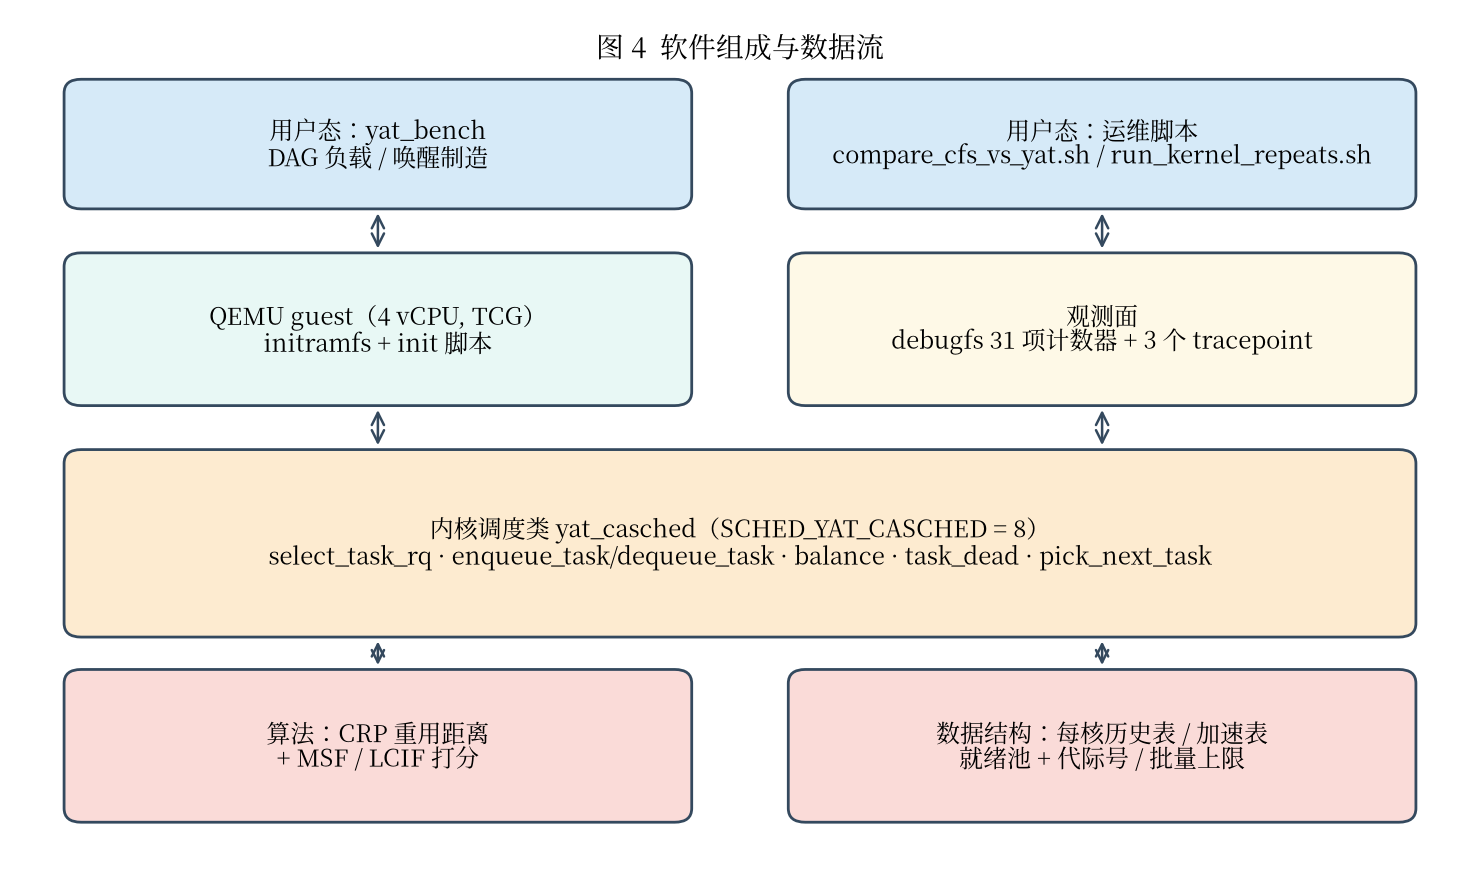
\includegraphics[width=0.86\textwidth]{figures/fig4-arch.png}
\caption{软件组成与数据流}
\label{fig:arch}
\end{figure}

\subsection{调度类回调与触发时机}

调度类通过实现一组回调接入内核调度器，见表 \ref{tab:callbacks}。

\begin{table}[H]
\centering
\caption{实现的调度类回调}
\label{tab:callbacks}
\small
\begin{tabular}{@{}p{3.8cm}p{4.2cm}p{5.8cm}@{}}
\toprule
回调 & 触发时机 & 本软件的处理 \\
\midrule
\code{select\_task\_rq} & 任务被唤醒或新建、且可运行核数 $>1$ & 计算候选核的加速比与缓存冲击，选一个核并记录 \\
\code{enqueue\_task} & 任务进入运行队列 & 维护 \code{nr\_running}、绑定作业、记录亲和信息 \\
\code{dequeue\_task} & 任务离开运行队列 & 解除绑定，同步 \code{nr\_running} \\
\code{balance} & 调度点（持有 \code{rq\_lock}） & 就绪池批量放置；池空且无新就绪时走快速路径 \\
\code{task\_dead} & 任务退出 & 释放作业与历史记录（关中断区间内完成） \\
\code{pick\_next\_task} & 选择下一个运行的任务 & 按优先级与就绪顺序取，并核对绑定关系 \\
\bottomrule
\end{tabular}
\end{table}

\subsection{一次唤醒的处理流程}

\begin{enumerate}
  \item 任务因等待的事件到达被唤醒，内核进入调度类的 \code{select\_task\_rq}；
  \item 软件读取该任务所属作业的历史放置记录，计算"上次所在核"的重用距离；
  \item 若目标核当前空闲且允许，直接复用上次的核（记为"空闲复用"），不做完整计算；
  \item 否则在可运行核集合上计算每个候选核的加速比与缓存冲击，按 MSF/LCIF 打分选择；
  \item 决策写入作业的放置表，任务入队；若决策的核与实际运行的核一致，记为一次"接管成功"；
  \item 每个调度点还会进入 \code{balance}：如果就绪池里有作业且出现了新的就绪事件，成批放置；
        否则直接返回，不取全局锁。
\end{enumerate}

\subsection{容量上限与可预测性}

软件对所有在线结构都设了硬上限（表 \ref{tab:limits}），因此最坏开销不随负载形状失控。

\begin{table}[H]
\centering
\caption{关键上限}
\label{tab:limits}
\small
\begin{tabular}{@{}p{4.8cm}p{3.0cm}p{7.6cm}@{}}
\toprule
对象 & 上限 & 作用 \\
\midrule
每核历史表记录数 & 512 条 & 超出后一次裁掉 1/4，在锁外释放 \\
单次全量决策的最小间隔 & 1\,ms & 每个任务每秒最多 1000 次决策 \\
单轮 balance 放置作业数 & 256 个 & 防止单轮循环过长 \\
就绪池扫描 & 由代际号触发 & 无新就绪作业时不扫描、不取锁 \\
\bottomrule
\end{tabular}
\end{table}

\subsection{一次完整运行的时序}

以"跑一次对比"为例，从命令到结果的时间顺序如下：

\begin{enumerate}
  \item 宿主执行对比脚本，脚本解析参数并检查文件锁；
  \item 检查内核镜像与 initramfs 是否存在，缺失则先调用构建脚本；
  \item 启动第一个 QEMU 实例，guest 内核以 CFS 为默认策略，init 脚本设置亲和性并运行负载；
  \item 负载完成后 guest 打印工作量与墙钟，宿主机收集串口日志并解析；
  \item guest 关机退出，宿主机释放资源，随后启动第二个 QEMU 实例；
  \item 第二个实例以 Yat 策略运行同一负载，结束后打印计数器与结果；
  \item 宿主脚本解析两侧日志，计算墙钟比值与派生比例，输出汇总行；
  \item 若指定了重复次数，重复第 3--7 步，最后按配置汇总中位数与全距。
\end{enumerate}

两个实例必须串行执行：它们共用 \code{results/} 下的中间文件，并行会互相覆盖。

\section{安装与部署}

\subsection{依赖检查}

在开始之前确认工具链齐全：

\begin{shell}
gcc --version | head -1
make --version | head -1
qemu-system-x86_64 --version | head -1
python3 --version
\end{shell}

\subsection{编译内核}

进入内核目录编译，产物是 \code{arch/x86/boot/bzImage}（不要使用 \code{vmlinux}，
QEMU 无法直接加载未压缩的 ELF 内核）：

\begin{shell}
cd linux-6.8-main
make defconfig
scripts/config --enable CONFIG_SCHED_CLASS_YAT_CASCHED
make -j"$(nproc)" bzImage
ls -l arch/x86/boot/bzImage
\end{shell}

首次完整编译在内核源码树上通常需要十几分钟到半小时，取决于机器核数；之后只改调度类文件时，
\code{make bzImage} 只需重编一个目标文件并重新链接，通常在两分钟以内。若编译报
\code{implicit declaration}，通常是头文件的 \code{CONFIG} 保护没打开，检查配置项是否生效；
若报 \code{multiple definition}，通常是同一符号在多个文件中定义，用 \code{make symbol-check}
可以定位。

只编译调度类目标文件可以用更快的方式检查语法（约 1 分钟）：

\begin{shell}
make kernel-obj        # 等价于只编 kernel/sched/yat_casched.o
\end{shell}

\subsection{制作 initramfs 与测试程序}

测试程序与 init 脚本会被打进 initramfs，guest 启动后自动运行：

\begin{shell}
bash linux-6.8-main/yat_test_scripts/build_yat_simple_test.sh
bash linux-6.8-main/yat_test_scripts/create_test_initramfs.sh
\end{shell}

这一步会生成静态链接的负载程序（\code{yat\_bench}）与 \code{init}，并打包成 cpio 归档。

\subsection{启动虚拟机}

最简启动方式：

\begin{shell}
bash linux-6.8-main/yat_test_scripts/start_qemu_yat_test.sh
\end{shell}

其等价的核心参数如下，其中三处必须注意（表 \ref{tab:qemu}）：

\begin{shell}
qemu-system-x86_64 \
  -kernel arch/x86/boot/bzImage -initrd build/compare_initramfs.cpio.gz \
  -m 1024 -smp 4 -nographic -no-reboot -accel tcg \
  -append "console=ttyS0,115200 panic=1 nokaslr yatbench=yat benchmark=8,2000000,0,none,200"
\end{shell}

\begin{table}[H]
\centering
\caption{QEMU 关键参数}
\label{tab:qemu}
\small
\begin{tabular}{@{}p{4.6cm}p{9.4cm}@{}}
\toprule
参数 & 说明 \\
\midrule
\code{-kernel .../bzImage} & 必须用压缩内核镜像；用 \code{vmlinux} 会报缺少 PVH note 而失败 \\
\code{-smp 4} & 处理器个数；若只有 1 核，多核调度代码路径不会被触发 \\
不得添加 \code{acpi=off} & 关掉 ACPI 后 guest 只识别到 1 个 CPU（AP 无法枚举） \\
\code{-accel tcg} & 无硬件虚拟化时的纯软件模拟；也可换 \code{-accel kvm} 在支持的主机上加速 \\
\code{yatbench/benchmark} & 传给 guest init 的负载参数：策略、任务数、迭代数、亲和性、睡眠微秒 \\
\bottomrule
\end{tabular}
\end{table}

\subsection{安装成功的判断标准}

guest 串口输出中出现以下三类信息，说明安装成功：

\begin{shell}
nr_cpu_ids=4
YATDEBUG-BEGIN ... YATDEBUG-END
YATBENCH-EXIT sum_work_units=16000000
\end{shell}

其中 \code{nr\_cpu\_ids=4} 表示 4 个 CPU 都被识别；\code{sum\_work\_units} 必须与预期一致
（8 个任务 $\times$ 2\,000\,000 次迭代 = 16\,000\,000），否则说明负载没有跑完，数据不可用。

\section{快速开始}

\subsection{跑一次对比}

最常用的功能是把同一份负载分别交给 CFS 与本软件，得到两者的墙钟比值：

\begin{shell}
bash linux-6.8-main/yat_test_scripts/compare_cfs_vs_yat.sh \
  --tasks 8 --iters 2000000 --kernel linux-6.8-main/arch/x86/boot/bzImage \
  --timeout 300 --affinity none --sleep-us 200
\end{shell}

脚本会先启动一次 CFS 的 guest，再启动一次 Yat 的 guest，最后打印：

\begin{shell}
sum_wall_ns     1460006170       2645705920
sum_wall 比 (yat/cfs): 1.8121   （<1 表示 Yat 更快）
\end{shell}

\subsection{查看计数器}

进入 guest 后可以直接读取调试接口。宿主侧也可以在启动脚本里把该文件打印到串口：

\begin{shell}
cat /sys/kernel/debug/yat_casched/stats
\end{shell}

输出为"名称 + 数值"的纯文本，每行一项，可直接用 \code{grep}、\code{awk} 处理。典型片段：

\begin{shell}
balance_runs      9
balance_noop      621
jobs_placed       172
select_calls      467
select_sticky_idle 295
ttwu_ok           512
nr_cpu_ids        4
\end{shell}

\subsection{跑重复测量并汇总}

单次结果受模拟器抖动影响，正式结论用 5 次重复的中位数与全距：

\begin{shell}
bash scripts/run_kernel_repeats.sh --repeats 5 \
     --out docs/validation/2026-11-13/kernel/repeat-routeA
cat docs/validation/2026-11-13/kernel/repeat-routeA/SUMMARY.txt
\end{shell}

汇总表格式如下（每行一组配置）：

\begin{shell}
config                n     median        min        max
none-sleep200         5      1.812      1.756      2.131
shared-sleep200       5      1.718      1.641      1.804
none-sleep0           5      0.838      0.812      1.171
\end{shell}

脚本内置文件锁：同一时刻只允许一个测量实例运行，第二个实例会直接退出并提示锁路径，
避免两个实例共用 \code{results/} 目录互相覆盖日志。
\subsection{运行产物}

一次测量会在输出目录下产生下列文件，它们是后续核对与归档的依据（\autoref{tab:artifacts}）。

\begin{table}[H]
\centering
\caption{运行产物}
\label{tab:artifacts}
\small
\begin{tabular}{@{}p{4.6cm}p{9.4cm}@{}}
\toprule
文件 & 内容 \\
\midrule
\code{run-N.csv} & 第 N 次运行的逐策略记录：标签、策略、墙钟、工作量、上下文切换、比值 \\
\code{run-N.log} & 第 N 次运行的完整串口输出，含计数器与负载结果 \\
\code{all.csv} & 全部运行的合并表，可直接用表格软件打开 \\
\code{SUMMARY.txt} & 按配置汇总的中位数、最小值、最大值 \\
\code{build/} & 中间产物：静态链接的负载程序与 initramfs 归档 \\
\bottomrule
\end{tabular}
\end{table}

归档时应当整目录保留，只保留 CSV 会丢失计数器与告警信息，事后无法判断数据是否可信。

\section{功能详解}

\subsection{缓存感知选核}

选核的输入有三样：任务的作业标识（\code{dag\_id}）、该作业的历史放置记录、各 CPU 的当前负载。
输出是一个 CPU 编号。处理分三步：

\begin{enumerate}
  \item \textbf{估计命中级别}：用上次放置到本次唤醒之间的时间间隔（重用距离）与每核历史表中记录
        的执行区间比较，得到"完全命中 / 部分命中 / 完全冷"三级；
  \item \textbf{计算加速比}：以命中级别对应的收益系数乘上任务的历史执行时长，得到该候选核下的
        预计加速比；
  \item \textbf{两条规则取优}：先按 MSF（最大加速比）排序，若多个核的预计收益接近，再由 LCIF
        （最小缓存冲击）在它们之中选择对其他作业影响最小的核。
\end{enumerate}

打分函数的形式如下（用文字表述，便于核对实现）：对每个候选核 $k$，先按其命中级别取
收益系数 $\eta\in[0,1]$，再乘以该任务的历史执行时长 $\hat{C}$ 得到预计节省时间；把节省时间
与该核当前负载 $\ell_k$ 合成加速比
\[ \mathrm{benefit}(k)=\frac{\hat{C}\cdot\eta}{\hat{C}+\ell_k}, \]
按 benefit 降序取第一；当第二名与第一名的 benefit 之差小于阈值时，改按"缓存冲击"选——
冲击定义为该核上已驻留的其他作业数量，取最小者。两条规则合并后即 MSF/LCIF。

选核结果会同时记入三处：作业的放置表（供后续比对）、每核历史表（供下一次估计）、
计数器（供用户核对）。如果候选集中没有可用的核，决策记为"无核可用"，任务仍会入队，
由后续调度点重试。

\subsection{作业与 DAG 生命周期}

作业（job）是调度的基本单位，一个作业对应 DAG 中的一个节点。状态与迁移见表 \ref{tab:states}。

\begin{table}[H]
\centering
\caption{作业状态与迁移}
\label{tab:states}
\small
\begin{tabular}{@{}p{2.6cm}p{5.0cm}p{6.8cm}@{}}
\toprule
状态 & 含义 & 迁移条件 \\
\midrule
新建 & 作业已创建，前驱未全部完成 & 创建时若前驱计数为 0，直接进入就绪 \\
就绪 & 可以运行，等待放置 & 被 \code{balance} 或选核取走时进入运行 \\
运行 & 已绑定任务并放到某个 CPU & 任务阻塞（睡眠）或完成时离开运行态 \\
完成 & 任务执行完毕 & 递减后继的前驱计数；计数归零者转为就绪 \\
销毁 & 作业释放 & 任务退出时的 \code{task\_dead} \\
\bottomrule
\end{tabular}
\end{table}

前驱计数归零是"作业变成就绪"的唯一条件，也是后文代际号自增的两个时机之一。

\subsection{就绪池与就绪代际门禁（V1.0 新增）}

就绪池保存所有"可以运行但还没被放置"的作业。早期版本在每个调度点都无条件扫描全部 DAG、
遍历其中所有作业，无论池中是否真的有新东西；在 8 任务、512 次唤醒的负载下，这种扫描发生了
757 次，而真正需要处理的只有其中一小部分。

V1.0 引入"就绪代际号"：

\begin{itemize}
  \item 维护一个全局计数器，记录"发生过多少次作业变成就绪的事件"；
  \item 事件有两个来源：作业创建时前驱计数为 0；某作业完成使后继的前驱计数降到 0；
  \item \code{balance} 只在代际号变化时扫描就绪池，并把"已扫描到的代际"推进到当前值；
  \item 池为空且代际未变时，\code{balance} 在取全局锁之前直接返回，只累加一个计数器。
\end{itemize}

代际号用的是原子加一，而不是锁保护的计数：加一发生在作业创建与作业完成的路径上，
这两处已经持有各自的锁，再套一层全局锁会引入新的锁序问题。原子变量只被读取用于比较，
不参与资源分配，因此即使读到稍旧的值，后果也只是"多扫描一次"，不会漏作业。

这条快速路径是保守的：只要池中还有作业（包括因找不到合适 CPU 而被放回的作业），
就永远不会走快速路径。效果见\autoref{fig:balance}：全量扫描从 757 次降到 9 次，
621 次调用变成不取锁的空转。

\begin{figure}[htbp]
\centering
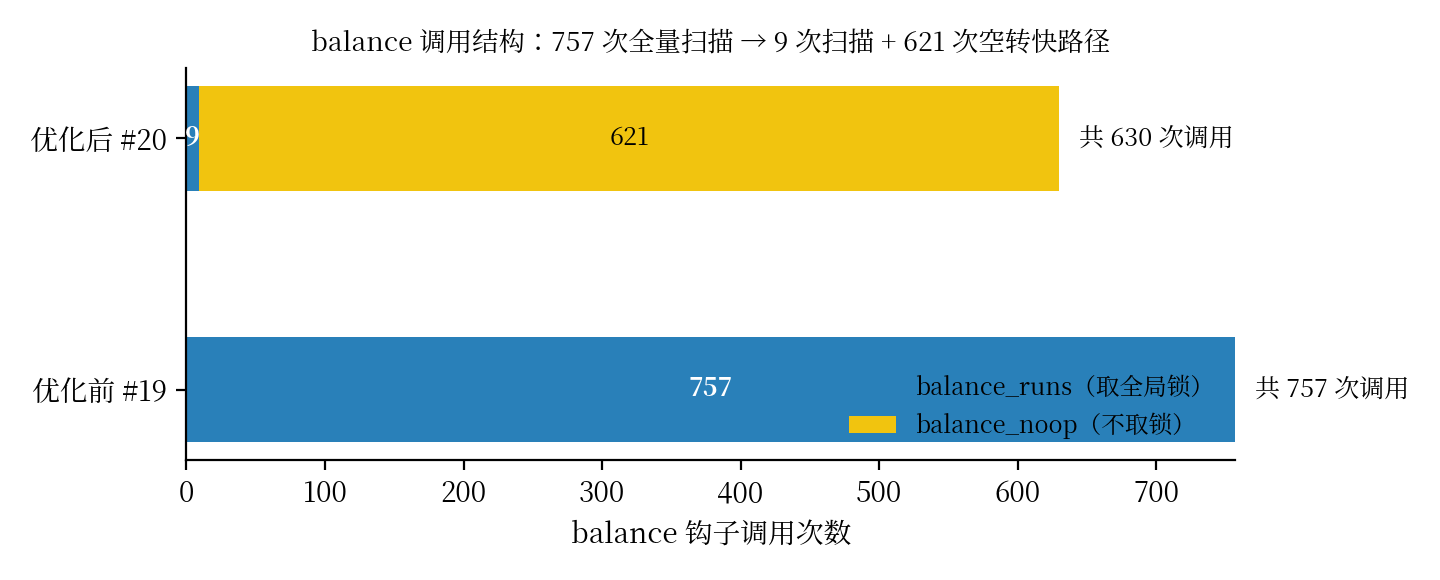
\includegraphics[width=0.86\textwidth]{figures/fig3-balance.png}
\caption{balance 调用结构的前后对比}
\label{fig:balance}
\end{figure}

\subsection{每核历史表与重用距离估计}

每个 CPU 维护一条历史记录链表，元素是"某作业在某段时间内于本核执行的区间"。查询时按作业
标识找到最近的记录，与当前时间比较得到重用距离。为避免内存无界增长，每条链表的记录数上限
为 512 条，超出后一次裁掉四分之一，被裁掉的元素在锁外释放。

该表直接决定了选核质量：记录越准，"这个作业的数据还在不在这个核"的判断越可靠。

\subsection{运行时可观测性}

软件提供 31 项计数器，通过 \code{debugfs} 暴露为纯文本，见表 \ref{tab:counters}。
它们的设计目的不是"展示"，而是让每一条关于系统的判断都有对应的读数。

\begin{table}[H]
\centering
\caption{主要计数器（分组）}
\label{tab:counters}
\small
\begin{tabular}{@{}p{4.4cm}p{3.0cm}p{7.0cm}@{}}
\toprule
计数器 & 组 & 用途 \\
\midrule
\code{ttwu\_ok} & 唤醒 & 成功唤醒次数，是其他比例的基数 \\
\code{select\_calls} & 选核 & 进入调度类的次数；为 0 说明亲和性把回调挡住了 \\
\code{select\_sticky\_idle} & 选核 & 目标核空闲、直接复用上次核的次数 \\
\code{select\_decided} & 选核 & 走完整打分的次数，应与 \code{jobs\_placed} 一致 \\
\code{place\_hit / miss / pending} & 落地 & 决策的核与实际运行核的比对，得出接管率 \\
\code{balance\_runs / noop} & 均衡 & 取锁扫描次数 / 池空空转次数 \\
\code{pool\_scans / skips} & 均衡 & 就绪池真实扫描次数 / 代际未变跳过次数 \\
\code{enq\_calls / enq\_cpus\_allowed} & 入队 & 后者除以前者即平均可运行核数 \\
\code{history\_records / accel\_inserts} & 数据 & 历史表规模与加速表更新次数 \\
\code{pick\_calls / pick\_null\_desync} & 选任务 & 后者非 0 表示运行计数维护有误 \\
\bottomrule
\end{tabular}
\end{table}

三个 tracepoint 用于带参数的离线分析（事件名以 \code{yat\_casched:} 开头），
分别对应"选核决策""作业进出就绪池""放置落地"。它们的开销高于计数器，
默认只在需要定位问题时打开。

\subsection{亲和性与自检}

任务的亲和性会直接决定 \code{select\_task\_rq} 是否被调用，因此软件把亲和性作为一等语义处理：

\begin{itemize}
  \item \code{shared}：全部任务绑定到同一核，可运行核数为 1，调度类回调不会被调用；
  \item \code{none}：不设绑定，任务可跨核，是选核功能的真实场景；
  \item \code{spread}：第 $i$ 个任务绑定到第 $i \bmod m$ 个核，用于观察任务是否被重新收敛。
\end{itemize}

自检程序 \code{yat\_affinity\_test} 在 guest 内直接验证"调度类返回的核落在允许掩码内"，
并在三个阶段分别打印实际核编号，通过时输出：

\begin{shell}
YAT-AFFINITY PASS rc=0
\end{shell}

\subsection{负载程序与对比工具}

\code{yat\_bench} 是自带的负载程序，参数含义见表 \ref{tab:bench}。它按"任务数 $\times$ 迭代数"
产生固定工作量的计算，并按设定睡眠间隔制造阻塞与唤醒，结束时打印完成的工作量，供两策略核对。

\begin{table}[H]
\centering
\caption{yat\_bench 参数}
\label{tab:bench}
\small
\begin{tabular}{@{}p{3.6cm}p{2.6cm}p{8.2cm}@{}}
\toprule
参数 & 取值示例 & 说明 \\
\midrule
任务数 & 8 & 每个任务对应一个作业 \\
迭代数 & 2000000 & 单任务工作量，8 任务合计 1600 万 \\
亲和性 & none & none / shared / spread \\
睡眠间隔 & 200 & 单位微秒；0 表示不制造唤醒 \\
策略 & yat & yat / cfs，由 init 在启动时切换 \\
\bottomrule
\end{tabular}
\end{table}

\subsection{编译期与运行期配置}

影响行为的常量与开关见\autoref{tab:config}。它们都在源码中显式命名，不使用魔法数。

\begin{table}[H]
\centering
\caption{主要配置项}
\label{tab:config}
\footnotesize
\begin{tabular}{@{}p{5.2cm}p{5.6cm}p{4.4cm}@{}}
\toprule
名称 & 位置 & 作用 \\
\midrule
\code{CONFIG\_SCHED\_...\_CASCHED} & 内核配置 & 是否把该调度类编入内核 \\
策略号 8 & \code{include/uapi/linux/sched.h} & 与用户态约定的策略编号 \\
\code{YAT\_HISTORY\_MAX\_RECORDS} & 调度类源码 & 每核历史表上限（512） \\
\code{YAT\_DECISION\_MIN\_INTERVAL\_NS} & 调度类源码 & 两次全量决策的最小间隔（1\,ms） \\
\code{YAT\_BALANCE\_MAX\_BATCH} & 调度类源码 & 单轮均衡最大放置数（256） \\
亲和性档位 & 负载参数 & \code{none} / \code{shared} / \code{spread} \\
睡眠间隔 & 负载参数 & 制造唤醒；为 0 时不产生唤醒 \\
\bottomrule
\end{tabular}
\end{table}

三个常量的取值都有明确理由：历史表 512 条是在"能覆盖一个作业的多次执行区间"与"每条链表
查找开销可接受"之间取的值，超出后一次裁掉 1/4 而不是逐条删除，避免在热路径上做链表遍历；
决策间隔 1 毫秒使单个任务每秒最多产生 1000 次决策，把最坏情况下的决策开销限定在每秒毫秒级；
单轮放置上限 256 个作业，保证一次 \code{balance} 的循环时间有界，不会因为池中积压而长时间
占用运行队列锁。

修改这些常量后必须重新编译内核并重建镜像；只改负载参数则无需重编。

\section{结果解读与验证}

\subsection{三组配置的含义}

同样的负载在三种配置下各跑一次，得到的比值回答三个不同的问题（\autoref{fig:three}）：

\begin{table}[H]
\centering
\caption{三组配置与判读}
\label{tab:three}
\small
\begin{tabular}{@{}p{4.4cm}p{2.4cm}p{7.6cm}@{}}
\toprule
配置 & 中位数 & 判读 \\
\midrule
\code{none} + 200\,$\mu$s & 1.81 & 完整链路（选核 + 接入）的总代价 \\
\code{shared} + 200\,$\mu$s & 1.72 & 回调一次不进，只剩"待在这个调度类里"的接入代价 \\
\code{none} + 无唤醒 & 0.84 & 只剩任务创建路径，差异落在噪声内 \\
\bottomrule
\end{tabular}
\end{table}

\begin{figure}[htbp]
\centering
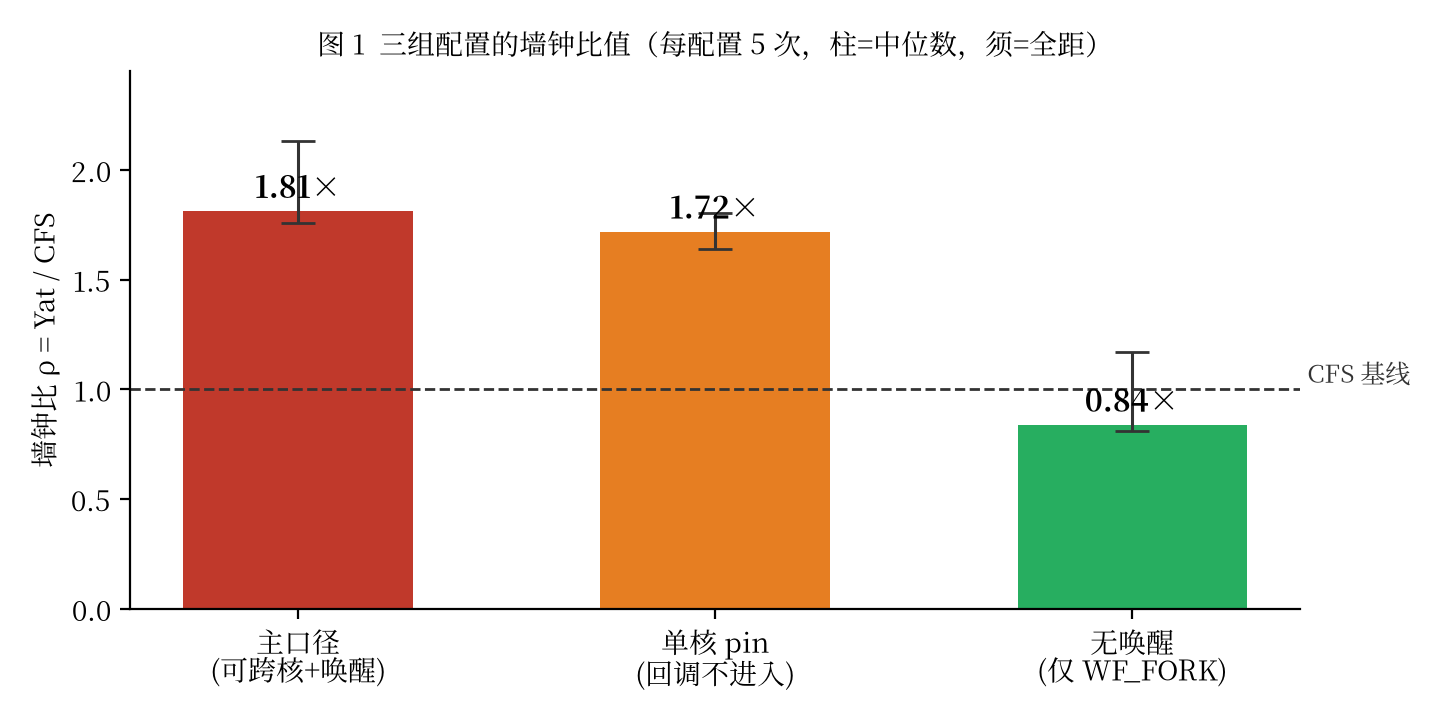
\includegraphics[width=0.80\textwidth]{figures/fig1-three-configs.png}
\caption{三组配置的墙钟比值（柱为 5 次中位数，须为全距）}
\label{fig:three}
\end{figure}

为什么用比值而不是绝对墙钟：模拟器上的绝对时间取决于宿主机的负载与调度，同一配置隔一天
重跑可以差出 20\% 以上；而同一批次内 CFS 与 Yat 两次运行共享同样的宿主状态，相除后大部分
系统误差被抵消。比值仍然有噪声，所以再叠加 5 次重复取中位数，把单次抖动压下去。

这三行必须一起读：第一行是总账，第二行把"选核"从总账里剥出去，两行之差说明选核本身的
边际代价；第三行用来确认代价确实随唤醒次数增长，而不是调度类的固定开销。

\subsection{版本间对比}

V1.0 相对上一版实现了就绪代际门禁，\autoref{fig:routea} 与表 \ref{tab:routea} 给出前后对比。

\begin{table}[H]
\centering
\caption{版本间关键指标对比}
\label{tab:routea}
\small
\begin{tabular}{@{}lccc@{}}
\toprule
指标 & 优化前 & 优化后（V1.0） & 变化 \\
\midrule
主口径墙钟比（中位数） & 2.00 & 1.81 & $-9.5\%$ \\
\code{balance\_runs} & 757 & 9 & $-98.8\%$ \\
\code{balance\_noop} & 无此计数 & 621 & 新增快路径 \\
\code{jobs\_placed} & 271 & 172 & 去掉无效重复放置 \\
接管率 & 97.9\% & 98.1\% & 持平 \\
\bottomrule
\end{tabular}
\end{table}

表中 \code{jobs\_placed} 从 271 降到 172 不是退步：旧实现每轮都把已经在睡眠的任务重新
"放置"一遍，这些放置不改变任何调度结果，只是把计数器撑大；新实现只放置真正需要放置的作业，
接管率反而从 97.9\% 升到 98.1\%。判断一个计数变小是好事还是坏事，要看它对应的行为是否产生
实际效果，而不是看数字大小。

\begin{figure}[H]
\centering
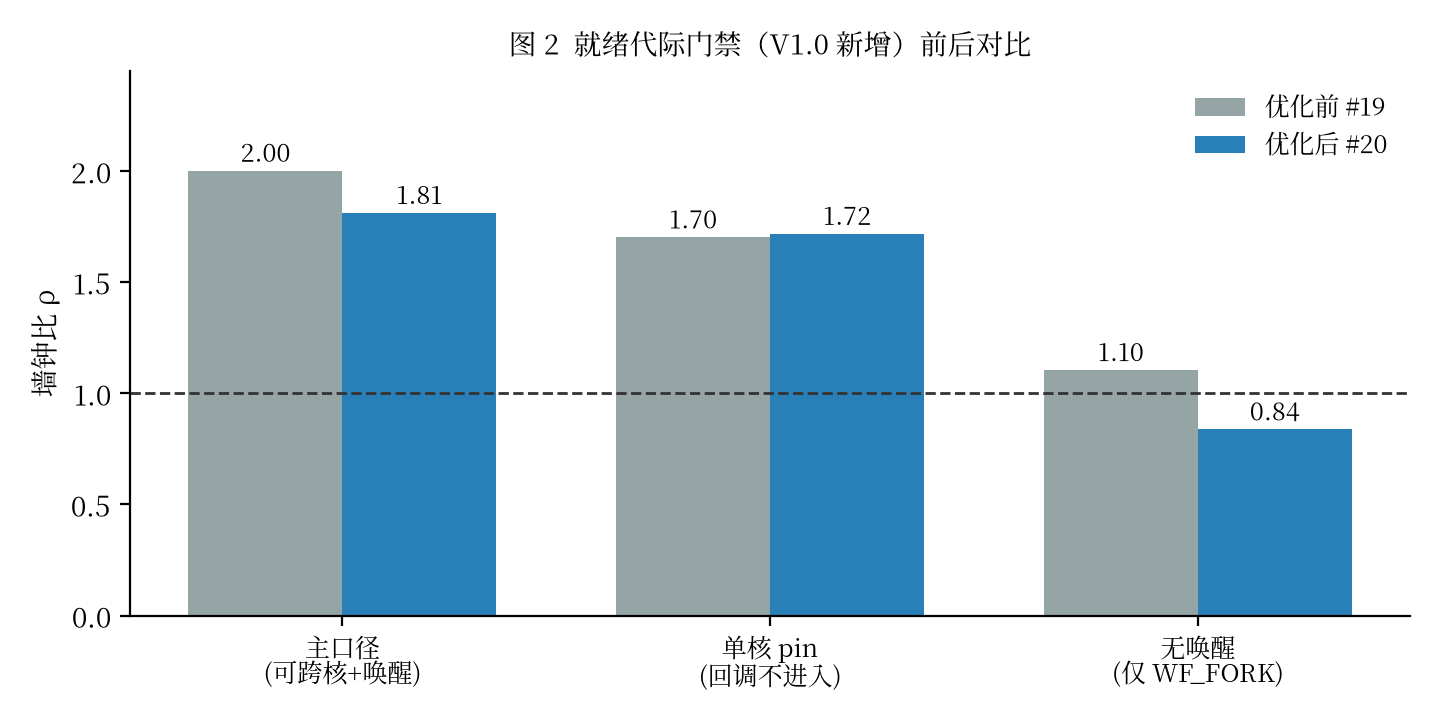
\includegraphics[width=0.80\textwidth]{figures/fig2-route-a.png}
\caption{就绪代际门禁前后对比（左柱为优化前，右柱为优化后）}
\label{fig:routea}
\end{figure}


\subsection{如何判断一次运行的数据可信}

按以下顺序核对，任一项不满足则应重跑：

\begin{enumerate}
  \item \code{sum\_work\_units} 是否等于预期（提示负载未跑完或提前退出）；
  \item \code{select\_calls} 是否大于 0（提示亲和性设置错误，回调根本没进）；
  \item \code{select\_decided} 与 \code{jobs\_placed} 是否一致（提示决策未落地）；
  \item \code{place\_hit} 与 \code{place\_pending} 的比例是否在 95\% 以上（提示放置表错乱）；
  \item \code{pick\_null\_desync} 是否为 0（非 0 表示运行计数维护有误）。
\end{enumerate}

\subsection{一键门禁}

仓库提供静态门禁，一条命令检查符号一致性、补丁完整性、文档链接与文档中的数字：

\begin{shell}
make verify-all
\end{shell}

全部通过时最后一行输出"全部门禁通过"；任意一项不通过都会列出具体条目并以非零状态退出。
其中 \code{make numbers-check} 会把文档里引用的数字与归档数据逐项比对，避免抄写错误进入材料。
\subsection{数据归档与复现口径}

为了让结果可被第三方复核，软件约定三条口径：

\begin{enumerate}
  \item \textbf{成对测量}：同一配置下先跑 CFS 再跑 Yat，两者使用同一镜像、同一负载参数、
        同一完成工作量；比值只在成对数据之间计算，不跨批次比较；
  \item \textbf{重复与统计量}：每配置至少 5 次重复，报中位数与全距；不报单次最优值，
        不把 5\% 量级的差异写成结论；
  \item \textbf{归档不裁剪}：CSV 与串口日志整目录保存，计数器与告警一并保留，
        以便他人判断数据是否满足使用条件。
\end{enumerate}

仓库中的 \code{make numbers-check} 会按这三条口径，把文档里出现的数字与归档数据逐项比对；
数字对不上时命令以非零状态退出。这样做的目的是让"文档写的"与"数据记的"不能悄悄分叉。

\section{常见问题与排错}

\begin{table}[H]
\centering
\caption{常见现象、原因与处置}
\label{tab:faq}
\small
\begin{tabular}{@{}p{4.6cm}p{4.6cm}p{5.2cm}@{}}
\toprule
现象 & 原因 & 处置 \\
\midrule
启动即退出，报 "Error loading uncompressed kernel without PVH ELF Note" &
使用了 \code{vmlinux} & 改用 \code{arch/x86/boot/bzImage} \\
guest 内 \code{nr\_cpu\_ids=1} & 启动参数里带了 \code{acpi=off} &
去掉 \code{acpi=off}/\code{noapic}，保留 ACPI \\
\code{select\_calls=0} 而 \code{enq\_calls} 正常 &
任务被绑定到单核，包装层直接返回 & 改用 \code{--affinity none} \\
串口出现 \code{possible irq lock inversion} &
池锁与运行队列锁的获取顺序不一致 & 升级到含修复的版本（补丁 0007） \\
日志里找不到 \code{YATCSV} 行且两次运行结果相同 &
两个测量实例并行，共用 \code{results/} 目录 & 等待前一个实例结束；脚本已加文件锁 \\
杀进程后残留 QEMU 占满 CPU & 中断导致子进程未回收 & \code{pkill -f qemu-system} 后重跑 \\
\code{make verify-all} 报数字不一致 &
文档里的数字与归档数据不符 & 以归档 CSV 为准修改文档，不要改门禁 \\
\bottomrule
\end{tabular}
\end{table}

补充说明两条容易误判的情况：

第一，"没有唤醒时看起来更快"不构成结论。该配置下比值的全距跨越 1，说明差异在噪声之内，
只能说明基础调度路径没有可测的额外开销，不能说明本软件更快。

第二，"某个版本单次跑出更低数字"不构成结论。同一配置连续三次运行的墙钟可相差约 28\%，
判断版本优劣要看 5 次重复的中位数与全距，而判断功能是否生效要看计数器。

\section{版本与维护}

\subsection{版本记录}

\begin{table}[H]
\centering
\caption{版本记录}
\label{tab:versions}
\small
\begin{tabular}{@{}p{2.2cm}p{3.4cm}p{8.6cm}@{}}
\toprule
版本 & 日期 & 主要变更 \\
\midrule
V1.0 & 2026-11-16 & 首个登记版本：调度类完整实现、31 项计数器、
就绪代际门禁、成对对比与重复测量工具、静态门禁 \\
\bottomrule
\end{tabular}
\end{table}

\subsection{补丁包与升级}

内核侧的改动以补丁形式提供，按序应用即可重建当前源码树：

\begin{shell}
bash scripts/kernel-patch.sh --check      # 校验补丁完整性与校验和
bash scripts/kernel-patch.sh --apply      # 应用到 linux-6.8-main/
bash scripts/kernel-patch.sh --status     # 查看每个补丁是否已应用
\end{shell}

补丁共 8 个，覆盖：调度类骨架与核心逻辑、内核接入点、文档、测试环境、锁序修复、
就绪代际门禁等。应用顺序由 \code{patches/series} 定义，不应调整。

\subsection{目录结构}

\begin{table}[H]
\centering
\caption{主要目录（未标前缀者均位于 \code{linux-6.8-main/} 下）}
\label{tab:dirs}
\small
\begin{tabular}{@{}p{3.9cm}p{10.1cm}@{}}
\toprule
目录 & 内容 \\
\midrule
\code{kernel/sched/} & 调度类实现（\code{yat\_casched.c}，约 2800 行） \\
\code{include/linux/sched/} & 对外声明头文件（29 个声明） \\
\code{include/trace/events/} & 3 个 tracepoint 的定义 \\
\code{boot\_test\_scripts/} & 负载程序、亲和性自检程序与说明 \\
\code{yat\_test\_scripts/} & initramfs 制作、QEMU 启动、成对对比脚本 \\
\code{scripts/}（仓库根） & 重复测量、数字核对、文档与符号门禁脚本 \\
\code{patches/}（仓库根） & 8 个可独立应用的补丁与校验和清单 \\
\code{docs/validation/}（仓库根） & 实测归档：CSV、串口日志、汇总表 \\
\bottomrule
\end{tabular}
\end{table}

\appendix

\section{命令速查}

\begin{table}[H]
\centering
\caption{常用命令}
\label{tab:cmds}
\small
\begin{tabular}{@{}p{7.2cm}p{6.8cm}@{}}
\toprule
命令 & 用途 \\
\midrule
\code{make kernel-obj} & 只编译调度类目标文件（快速语法检查） \\
\code{make kernel-build} & 编译内核并产出 \code{bzImage} \\
\code{make symbol-check} & 校验头文件声明与实现一一对应 \\
\code{make patch-check} & 校验补丁完整性与校验和 \\
\code{make numbers-check} & 校验文档数字与归档数据一致 \\
\code{make docs-check} & 校验文档内部链接 \\
\code{make verify-all} & 运行以上全部门禁 \\
\code{bash scripts/run\_kernel\_repeats.sh --repeats 5 --out DIR} & 重复测量并汇总 \\
\code{bash .../compare\_cfs\_vs\_yat.sh --help} & 查看成对对比脚本参数 \\
\bottomrule
\end{tabular}
\end{table}

\section{典型输出样例}

一次完整对比运行中，CFS 与 Yat 两侧的汇总行如下（数值取自归档日志）：

\begin{shell}
[CFS] sum_work_units = 16000000   vol_ctx = 472   invol_ctx = 133
[Yat] sum_work_units = 16000000   vol_ctx = 467   invol_ctx = 80
sum_wall_ns     1460006170       2645705920
sum_wall 比 (yat/cfs): 1.8121
\end{shell}

Yat 侧的计数器输出（节选）：

\begin{shell}
balance_runs      9
balance_skips     0
balance_noop      621
jobs_placed       172
jobs_nocore       0
history_records   824
select_calls      467
select_sticky_idle 295
select_decided    172
enq_calls         475
enq_cpus_allowed  1900
ttwu_ok           512
pick_calls        932
pick_null_desync  0
place_hit         906
place_miss        0
place_pending     18
nr_cpu_ids        4
\end{shell}

据此可以直接算出三个比例：唤醒进入调度类的比例 $467/512=91.2\%$、空闲复用比例
$295/467=63.2\%$、接管率 $906/(906+0+18)=98.1\%$。说明书中的这三处数字与
第 6 节的图表同源，均由归档 CSV 重算。

\end{document}